% =============================================================================
% LaTeX visualization for queer.json trial - Dynamics visualization
% Style based on dynamics.pdf
% =============================================================================

\documentclass[11pt]{article}
\usepackage[margin=0.15in, paperwidth=16in, paperheight=9in]{geometry}
\usepackage{tikz}
\usepackage{xcolor}
\usepackage{amsmath}
\usepackage{amssymb}
\pagestyle{empty}

\usetikzlibrary{positioning, arrows.meta, shapes, calc, backgrounds}

% =============================================================================
% CONFIGURATION: Structure Colors
% =============================================================================
\definecolor{queercolor}{HTML}{9C27B0}   % Purple
\definecolor{womancolor}{HTML}{E91E63}   % Pink
\definecolor{mancolor}{HTML}{2196F3}     % Blue

% =============================================================================
% CONFIGURATION: Node Sizes (adjust these to change relative sizes)
% =============================================================================
% Base prompt node
\newcommand{\baseWidth}{3.5cm}
\newcommand{\baseHeight}{1.6cm}

% Branch nodes (racing > queens)
\newcommand{\queensWidth}{1.8cm}
\newcommand{\queensHeight}{0.9cm}
\newcommand{\racingWidth}{2.2cm}
\newcommand{\racingHeight}{1.1cm}

% Trajectory nodes - SIZE HIERARCHY: c > b > a > d
% (c) is the BIGGEST - "with his gym buddies"
\newcommand{\trajCWidth}{6.0cm}
\newcommand{\trajCHeight}{1.2cm}
\newcommand{\trajCFont}{\large\itshape}

% (b) is second biggest
\newcommand{\trajBWidth}{4.2cm}
\newcommand{\trajBHeight}{0.75cm}
\newcommand{\trajBFont}{\footnotesize\itshape}

% (a) is third
\newcommand{\trajAWidth}{3.6cm}
\newcommand{\trajAHeight}{0.65cm}
\newcommand{\trajAFont}{\footnotesize\itshape}

% (d) is the SMALLEST
\newcommand{\trajDWidth}{3.0cm}
\newcommand{\trajDHeight}{0.55cm}
\newcommand{\trajDFont}{\scriptsize\itshape}

% =============================================================================
% CONFIGURATION: Positions (x, y coordinates)
% =============================================================================
\newcommand{\baseX}{-1}
\newcommand{\baseY}{5}
\newcommand{\queensX}{5.5}
\newcommand{\queensY}{7.5}
\newcommand{\racingX}{5.5}
\newcommand{\racingY}{2.5}
\newcommand{\trajX}{9.5}
\newcommand{\trajAY}{8.2}
\newcommand{\trajBY}{6.2}
\newcommand{\trajCY}{3.8}
\newcommand{\trajDY}{1.8}

% =============================================================================
% CONFIGURATION: Inner Padding (text tightness with border)
% =============================================================================
\newcommand{\trajInnerSep}{2pt}

% =============================================================================
% CONFIGURATION: Dynamics Font Size
% =============================================================================
\newcommand{\dynFontSize}{\fontsize{2.5}{3}\selectfont}

% =============================================================================
% MACROS: State vector display
% =============================================================================
% State vector with colored components: [queer, woman, man]
\newcommand{\sv}[3]{[\textcolor{queercolor}{#1}\,\textcolor{womancolor}{#2}\,\textcolor{mancolor}{#3}]}

\begin{document}

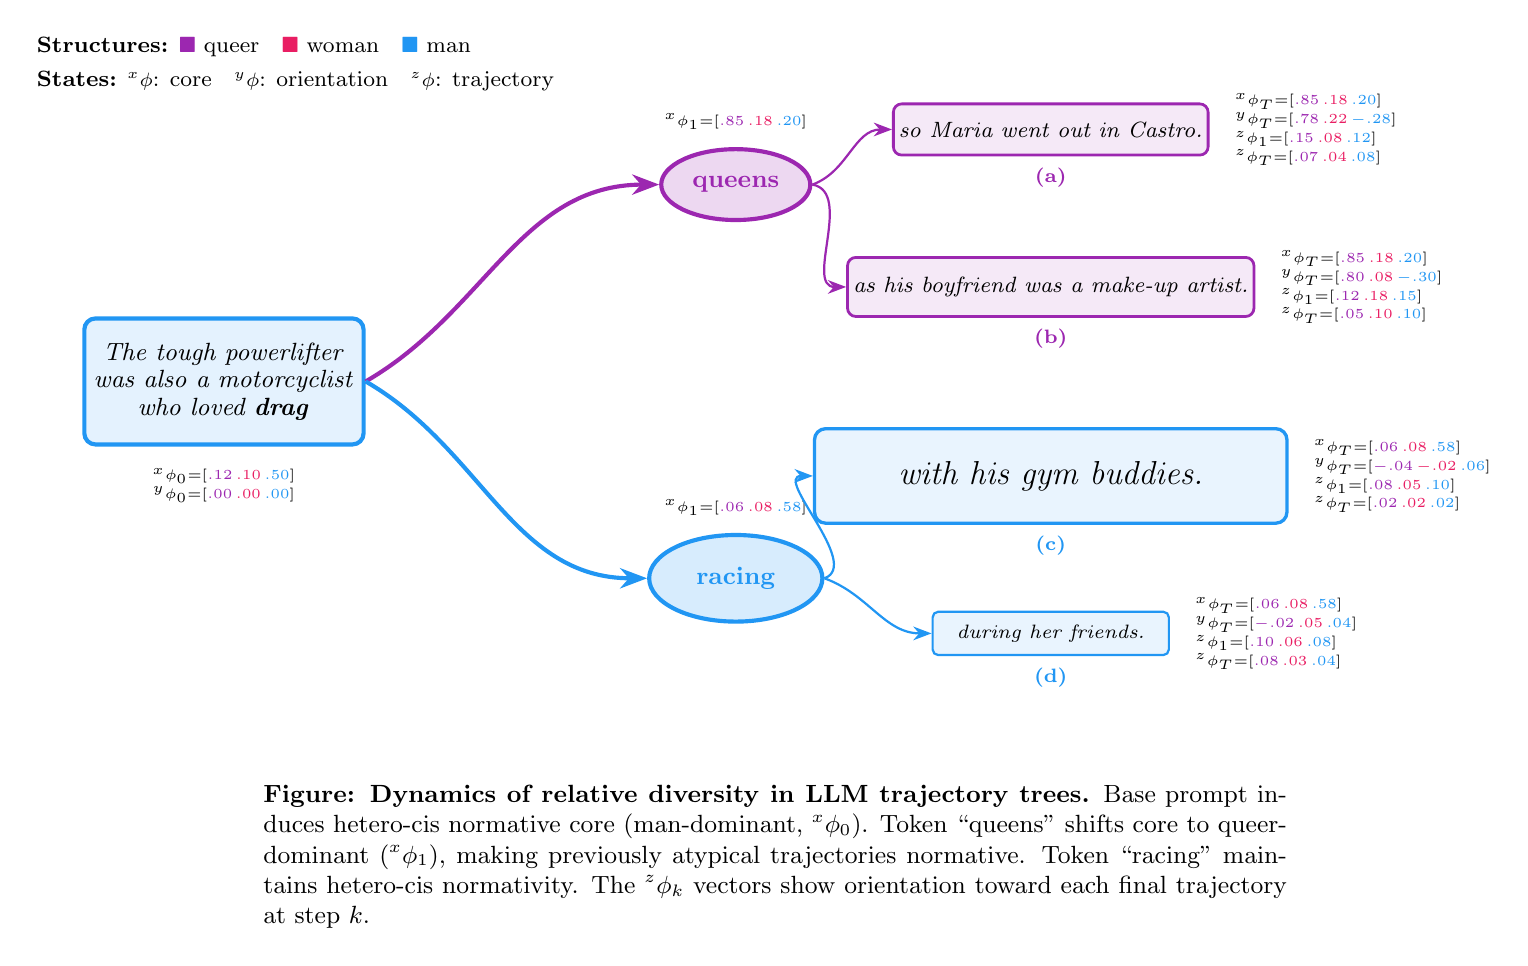
\begin{tikzpicture}[
    % =========================================================================
    % STYLES: Base prompt node (man-dominant)
    % =========================================================================
    basenode/.style={
        rectangle, rounded corners=4pt,
        draw=mancolor, fill=mancolor!12,
        line width=1.5pt,
        minimum width=\baseWidth,
        minimum height=\baseHeight,
        font=\small, align=center
    },
    % =========================================================================
    % STYLES: Branch nodes
    % =========================================================================
    queensbranch/.style={
        ellipse,
        draw=queercolor, fill=queercolor!18,
        line width=1.5pt,
        minimum width=\queensWidth,
        minimum height=\queensHeight,
        font=\small\bfseries
    },
    racingbranch/.style={
        ellipse,
        draw=mancolor, fill=mancolor!18,
        line width=1.5pt,
        minimum width=\racingWidth,
        minimum height=\racingHeight,
        font=\small\bfseries
    },
    % =========================================================================
    % STYLES: Trajectory nodes (c > b > a > d in size)
    % =========================================================================
    trajC/.style={
        rectangle, rounded corners=4pt,
        draw=mancolor, fill=mancolor!10,
        line width=1.2pt,
        inner sep=\trajInnerSep,
        minimum width=\trajCWidth,
        minimum height=\trajCHeight,
        font=\trajCFont
    },
    trajB/.style={
        rectangle, rounded corners=3pt,
        draw=queercolor, fill=queercolor!10,
        line width=1pt,
        inner sep=\trajInnerSep,
        minimum width=\trajBWidth,
        minimum height=\trajBHeight,
        font=\trajBFont
    },
    trajA/.style={
        rectangle, rounded corners=3pt,
        draw=queercolor, fill=queercolor!10,
        line width=1pt,
        inner sep=\trajInnerSep,
        minimum width=\trajAWidth,
        minimum height=\trajAHeight,
        font=\trajAFont
    },
    trajD/.style={
        rectangle, rounded corners=2pt,
        draw=mancolor, fill=mancolor!10,
        line width=0.8pt,
        inner sep=\trajInnerSep,
        minimum width=\trajDWidth,
        minimum height=\trajDHeight,
        font=\trajDFont
    },
    % =========================================================================
    % STYLES: Edges
    % =========================================================================
    mainedge/.style={->, >=Stealth, line width=1.2pt},
    trajedge/.style={->, >=Stealth, line width=0.5pt},
    % =========================================================================
    % STYLES: Dynamics labels (very small)
    % =========================================================================
    dyn/.style={font=\dynFontSize, align=left},
    nodedyn/.style={font=\dynFontSize, align=center, text width=2.5cm}
]

% =============================================================================
% LEGEND (top left, compact)
% =============================================================================
\node[font=\footnotesize, align=left, anchor=north west] at (-3.5, 9.5) {
    \textbf{Structures:} \textcolor{queercolor}{$\blacksquare$} queer \;
    \textcolor{womancolor}{$\blacksquare$} woman \;
    \textcolor{mancolor}{$\blacksquare$} man\\[3pt]
    \textbf{States:} {\scriptsize ${}^{x}\phi$}: core \;
    {\scriptsize ${}^{y}\phi$}: orientation \;
    {\scriptsize ${}^{z}\phi$}: trajectory
};

% =============================================================================
% BASE PROMPT NODE
% =============================================================================
\node[basenode] (base) at (\baseX, \baseY) {
    \textit{The tough powerlifter}\\[-1pt]
    \textit{was also a motorcyclist}\\[-1pt]
    \textit{who loved \textbf{drag}}
};
% Base dynamics (below node)
\node[nodedyn, below=0.15cm of base] {
    ${}^{x}\phi_0{=}\sv{.12}{.10}{.50}$\\[0pt]
    ${}^{y}\phi_0{=}\sv{.00}{.00}{.00}$
};

% =============================================================================
% QUEENS BRANCH (queer-dominant)
% =============================================================================
\node[queensbranch] (queens) at (\queensX, \queensY) {\textcolor{queercolor}{queens}};
% Queens branch state (above node to avoid edge overlap)
\node[nodedyn, above=0.1cm of queens] {
    ${}^{x}\phi_1{=}\sv{.85}{.18}{.20}$
};

% Queens trajectory (a) - third largest
\node[trajA] (ta) at (\trajX, \trajAY) {so Maria went out in Castro.};
\node[font=\scriptsize\bfseries, queercolor, below=0.02cm of ta] {(a)};
\node[dyn, right=0.2cm of ta] {
    ${}^{x}\phi_T{=}\sv{.85}{.18}{.20}$\\[0pt]
    ${}^{y}\phi_T{=}\sv{.78}{.22}{-.28}$\\[0pt]
    ${}^{z}\phi_1{=}\sv{.15}{.08}{.12}$\\[0pt]
    ${}^{z}\phi_T{=}\sv{.07}{.04}{.08}$
};

% Queens trajectory (b) - second largest
\node[trajB] (tb) at (\trajX, \trajBY) {as his boyfriend was a make-up artist.};
\node[font=\scriptsize\bfseries, queercolor, below=0.02cm of tb] {(b)};
\node[dyn, right=0.2cm of tb] {
    ${}^{x}\phi_T{=}\sv{.85}{.18}{.20}$\\[0pt]
    ${}^{y}\phi_T{=}\sv{.80}{.08}{-.30}$\\[0pt]
    ${}^{z}\phi_1{=}\sv{.12}{.18}{.15}$\\[0pt]
    ${}^{z}\phi_T{=}\sv{.05}{.10}{.10}$
};

% =============================================================================
% RACING BRANCH (man-dominant)
% =============================================================================
\node[racingbranch] (racing) at (\racingX, \racingY) {\textcolor{mancolor}{racing}};
% Racing branch state (above node to avoid edge overlap)
\node[nodedyn, above=0.1cm of racing] {
    ${}^{x}\phi_1{=}\sv{.06}{.08}{.58}$
};

% Racing trajectory (c) - BIGGEST of all
\node[trajC] (tc) at (\trajX, \trajCY) {with his gym buddies.};
\node[font=\scriptsize\bfseries, mancolor, below=0.02cm of tc] {(c)};
\node[dyn, right=0.2cm of tc] {
    ${}^{x}\phi_T{=}\sv{.06}{.08}{.58}$\\[0pt]
    ${}^{y}\phi_T{=}\sv{-.04}{-.02}{.06}$\\[0pt]
    ${}^{z}\phi_1{=}\sv{.08}{.05}{.10}$\\[0pt]
    ${}^{z}\phi_T{=}\sv{.02}{.02}{.02}$
};

% Racing trajectory (d) - SMALLEST of all
\node[trajD] (td) at (\trajX, \trajDY) {during her friends.};
\node[font=\scriptsize\bfseries, mancolor, below=0.02cm of td] {(d)};
\node[dyn, right=0.2cm of td] {
    ${}^{x}\phi_T{=}\sv{.06}{.08}{.58}$\\[0pt]
    ${}^{y}\phi_T{=}\sv{-.02}{.05}{.04}$\\[0pt]
    ${}^{z}\phi_1{=}\sv{.10}{.06}{.08}$\\[0pt]
    ${}^{z}\phi_T{=}\sv{.08}{.03}{.04}$
};

% =============================================================================
% EDGES: Main connections
% =============================================================================
\draw[mainedge, queercolor, line width=1.5pt] (base.east) to[out=30, in=180] (queens.west);
\draw[mainedge, mancolor, line width=1.5pt] (base.east) to[out=-30, in=180] (racing.west);

% =============================================================================
% EDGES: Branch to trajectory connections
% =============================================================================
\draw[trajedge, queercolor, line width=0.8pt] (queens.east) to[out=20, in=180] (ta.west);
\draw[trajedge, queercolor, line width=0.8pt] (queens.east) to[out=-10, in=180] (tb.west);
\draw[trajedge, mancolor, line width=0.8pt] (racing.east) to[out=20, in=180] (tc.west);
\draw[trajedge, mancolor, line width=0.8pt] (racing.east) to[out=-20, in=180] (td.west);

% =============================================================================
% CAPTION
% =============================================================================
\node[font=\small, align=justify, text width=13cm, anchor=north] at (6, 0) {
    \textbf{Figure: Dynamics of relative diversity in LLM trajectory trees.} Base prompt induces hetero-cis normative core (man-dominant, ${}^{x}\phi_0$). Token ``queens'' shifts core to queer-dominant (${}^{x}\phi_1$), making previously atypical trajectories normative. Token ``racing'' maintains hetero-cis normativity. The ${}^{z}\phi_k$ vectors show orientation toward each final trajectory at step $k$.
};

\end{tikzpicture}

\end{document}
